%
% Introduction to quantum information theory
%
\clearpage

\section{Introduction to quantum information theory}\index{Quantum information theory}


\famousquote{When you find yourself in a room surrounded by your enemies you tell yourself, `I am not locked in here with you, you are locked in here with me'. This is the kind of mindset you should have if you want to succeed in life. Get rid of that victim mentality.}{Bruce Lee}

\subsection{Probability, information and classical correlation measures}

% The fundamental unit in Shannon information is the \textit{bit}. 

``Information theory begins with the observation that there is a fundamental link between probabilities and information." 


With a given event (whose value is a random variable $X$), suppose that it has a set of outcomes $\{x\}$, each occuring with probability 
$\{p_x \}$. Then the \textit{Shannon entropy} associated with the random variable is defined as


\begin{align}\index{Shannon entropy}
H(X) = -\sum_x p_x\log_2(p_x).
\end{align}

Entropy plays a central role in information theory. The intuitive interpretation is that it quantifies an experimenter's uncertainty about $X$ before measuring it, and his expected information gain is $H(X)$ bits upon learning the outcome. The information $H(X)$ is zero if and only if one of the probabilities $p(x)$ is unity, with the others being zero. In this case the value of $X$ is already known and so there is no information to be gained from observing it.  

 If there are two random variables $X$ and $Y$, the joint entropy of the two is simply given by,
\begin{align}\index{Joint Shannon entropy}
H(X,Y) =  -\sum_{x,y} p_{x,y}\log_2(p_{x,y}).
\end{align}

Note that the joint entropy $H(X,Y)= H(X)+H(Y)$ if and only if $X$ and $Y$ are independent,i.e. the occurence of one does not change the probability of the other.  

\begin{figure}[hbt]
\includegraphics[clip=true, width=0.4\textwidth]{classical_mutual_info.pdf}
\captionspacefig \caption{\label{fig:mutual_info}}	
\end{figure}

If the two distributions are not independent, i.e. knowing something about $X$ reveals information on $U$, the two variables are said to be \textit{correlated}. Suppose Alice possesses the random variable $X$ and Bob has the random variable $Y$, the \textit{mutual information} specifies the number of bits in common between the two distributions. Equivalently, this represents the maximum number of bits that one party can learn about the other just by inspecting their own information.

For two classical distributions, the classical mutual information is given by,
\begin{align}\index{Mutual information}
I(X;Y) = H(X) + H(Y) - H(X,Y).
\label{classical_mutual_info}
\end{align}

It is a measure of the correlation between the events $X$ and $Y$. The quantity in Eq.~\eqref{classical_mutual_info} is important because it upper bounds the amount of information Alice and Bob can
reliably communicate. For a discrete random variable with $d$ possible outcomes, the maximum mutual information between $X$ and $Y$ is $I(X,Y)=\log_2 d$ bits.


Another quantity of interest is the \textit{conditional entropy}, which describes the entropy of $y$ should $X$ is known. The entropy of $Y$ conditioned on $X$ is given by
\begin{align}
H(X|Y) &= H(X,Y)- H(Y) \\
       &=- \sum_{x,y} p(x,y) \log_2 \frac{p(x,y)}{p(x)}.
\end{align}
\noindent Classically the conditional entropy is always positive, but as we will see later, this is not the case if quantum states are involved.

The relationship between the quantities mentioned above is graphically summarised in Figure~\ref{fig:mutual_info}.



% 
% 
% 
% 
% 

\subsection{Quantum correlation measures}

The von Neuman entropy\index{von Neuman entropy} \cite{bib:bengtsson2017geometry} for quantum density operators, $S(\hat\rho)$, is defined analogously, replacing probabilities with density operator eigenvalues,
\begin{align}\index{von Neuman entropy}
S(\hat\rho) &= - \sum_x \lambda_x \log_2 (\lambda_x) \nonumber \\
&= -\mathrm{tr}(\hat\rho\,\log \,\hat\rho),
\end{align}
where $\{\lambda\}$ is the eigenvalue spectrum of $\hat\rho$. This modification is logically justified, as the eigenvalues can be interpreted directly as a purely classical probability distribution of orthogonal states when the density operator is transformed into a basis with no coherences between basis states (i.e a diagonal basis or spectral decomposition\index{Spectral decomposition}). In that case, the Shannon and von Neuman entropies essentially have identical physical interpretations.

There are a few properties of the Von Neumann entropy which are often useful \cite{}:
\begin{enumerate}
	\item For pure states $\hat \rho = \ket{\psi}\bra{\psi}, S(\hat\rho) =0$.
	\item The Von Neumann entropy is unchanged by a unitary change of basis, 
			\begin{align}
			S(U\hat \rho U^\dagger) = S(\hat \rho)
			\end{align}
	\item For a state living on a Hilbert space of dimension $d$, $S(\hat\rho) \leq \log_2 d$, the equality is achieved when the quantum state is maximally mixed.
	\item For a given bipartite system $AB$
			\begin{align}
			S(\hat \rho_{AB}) \leq S(\hat \rho_A) + S(\hat \rho_B).
			\end{align}
			Equality holds if $\rho_{AB}= \rho_A \otimes \rho_B$.
\end{enumerate}



Analogously, the quantum mutual information\index{Quantum mutual information} for bipartite state $\hat\rho_{A,B}$ is defined as,
\begin{align}
I(A;B)_{\hat\rho} = S(\hat\rho_A) + S(\hat\rho_B) - S(\hat\rho_{A,B}),
\end{align}
using the von Neuman entropy.

The mutual information between two quantum states is invariant under local unitary transformations,
\begin{align}
I(A;B)_{\hat\rho} = I(\hat{U}_A\hat\rho_A \hat{U}_A^\dag; \hat{U}_B\hat\rho_B \hat{U}_B^\dag),
\end{align}
since the eigenvalue spectrum of a density operator is invariant under unitary transformations. Therefore, the mutual information represents the maximum amount of information Bob can learn about Alice's state under \textit{any} local operations.

Now, in sharp contrast with the classical case, the conditional entropy for quantum states
\begin{align}
H(A| B) = S(\hat \rho_{AB}) - S(\hat \rho_B)
\label{cond_quant_ent}
\end{align}
\noindent can be negative! If $\rho_{AB}$ is a maximally entangled state, then 
$S(\hat \rho_{AB}) =0$, and $H(A|B) =- S(\hat \rho_{AB}) <0$.
Intuitively, this can be interpreted as the fact that bipartite maximally entangled states can be more strongly correlated than classically possible, and that knowing the state of $A$ reveals an ``unnatural" amount of information about the state of $B$.






A quantum process cannot increase the mutual information between two parties. This yields the \textit{data processing inequality}\index{Data processing inequality} that, for a sequence of channels \mbox{$X\to Y\to Z$},
\begin{align}\index{Data processing inequality}\label{eq:data_proc_ineq}
I(X:Z)&\leq I(X:Y), \nonumber \\
I(X:Z)&\leq I(Y:Z),
\end{align}
with equality if and only if the channel not specified in the identity on the right hand side (\mbox{$Y\to Z$} or \mbox{$X\to Y$} respectively) is unitary, i.e one of the links in the chain perfectly preserves information content. The progression is shown in Fig.~\ref{fig:data_proc_ineq}.

\begin{figure}[!htbp]
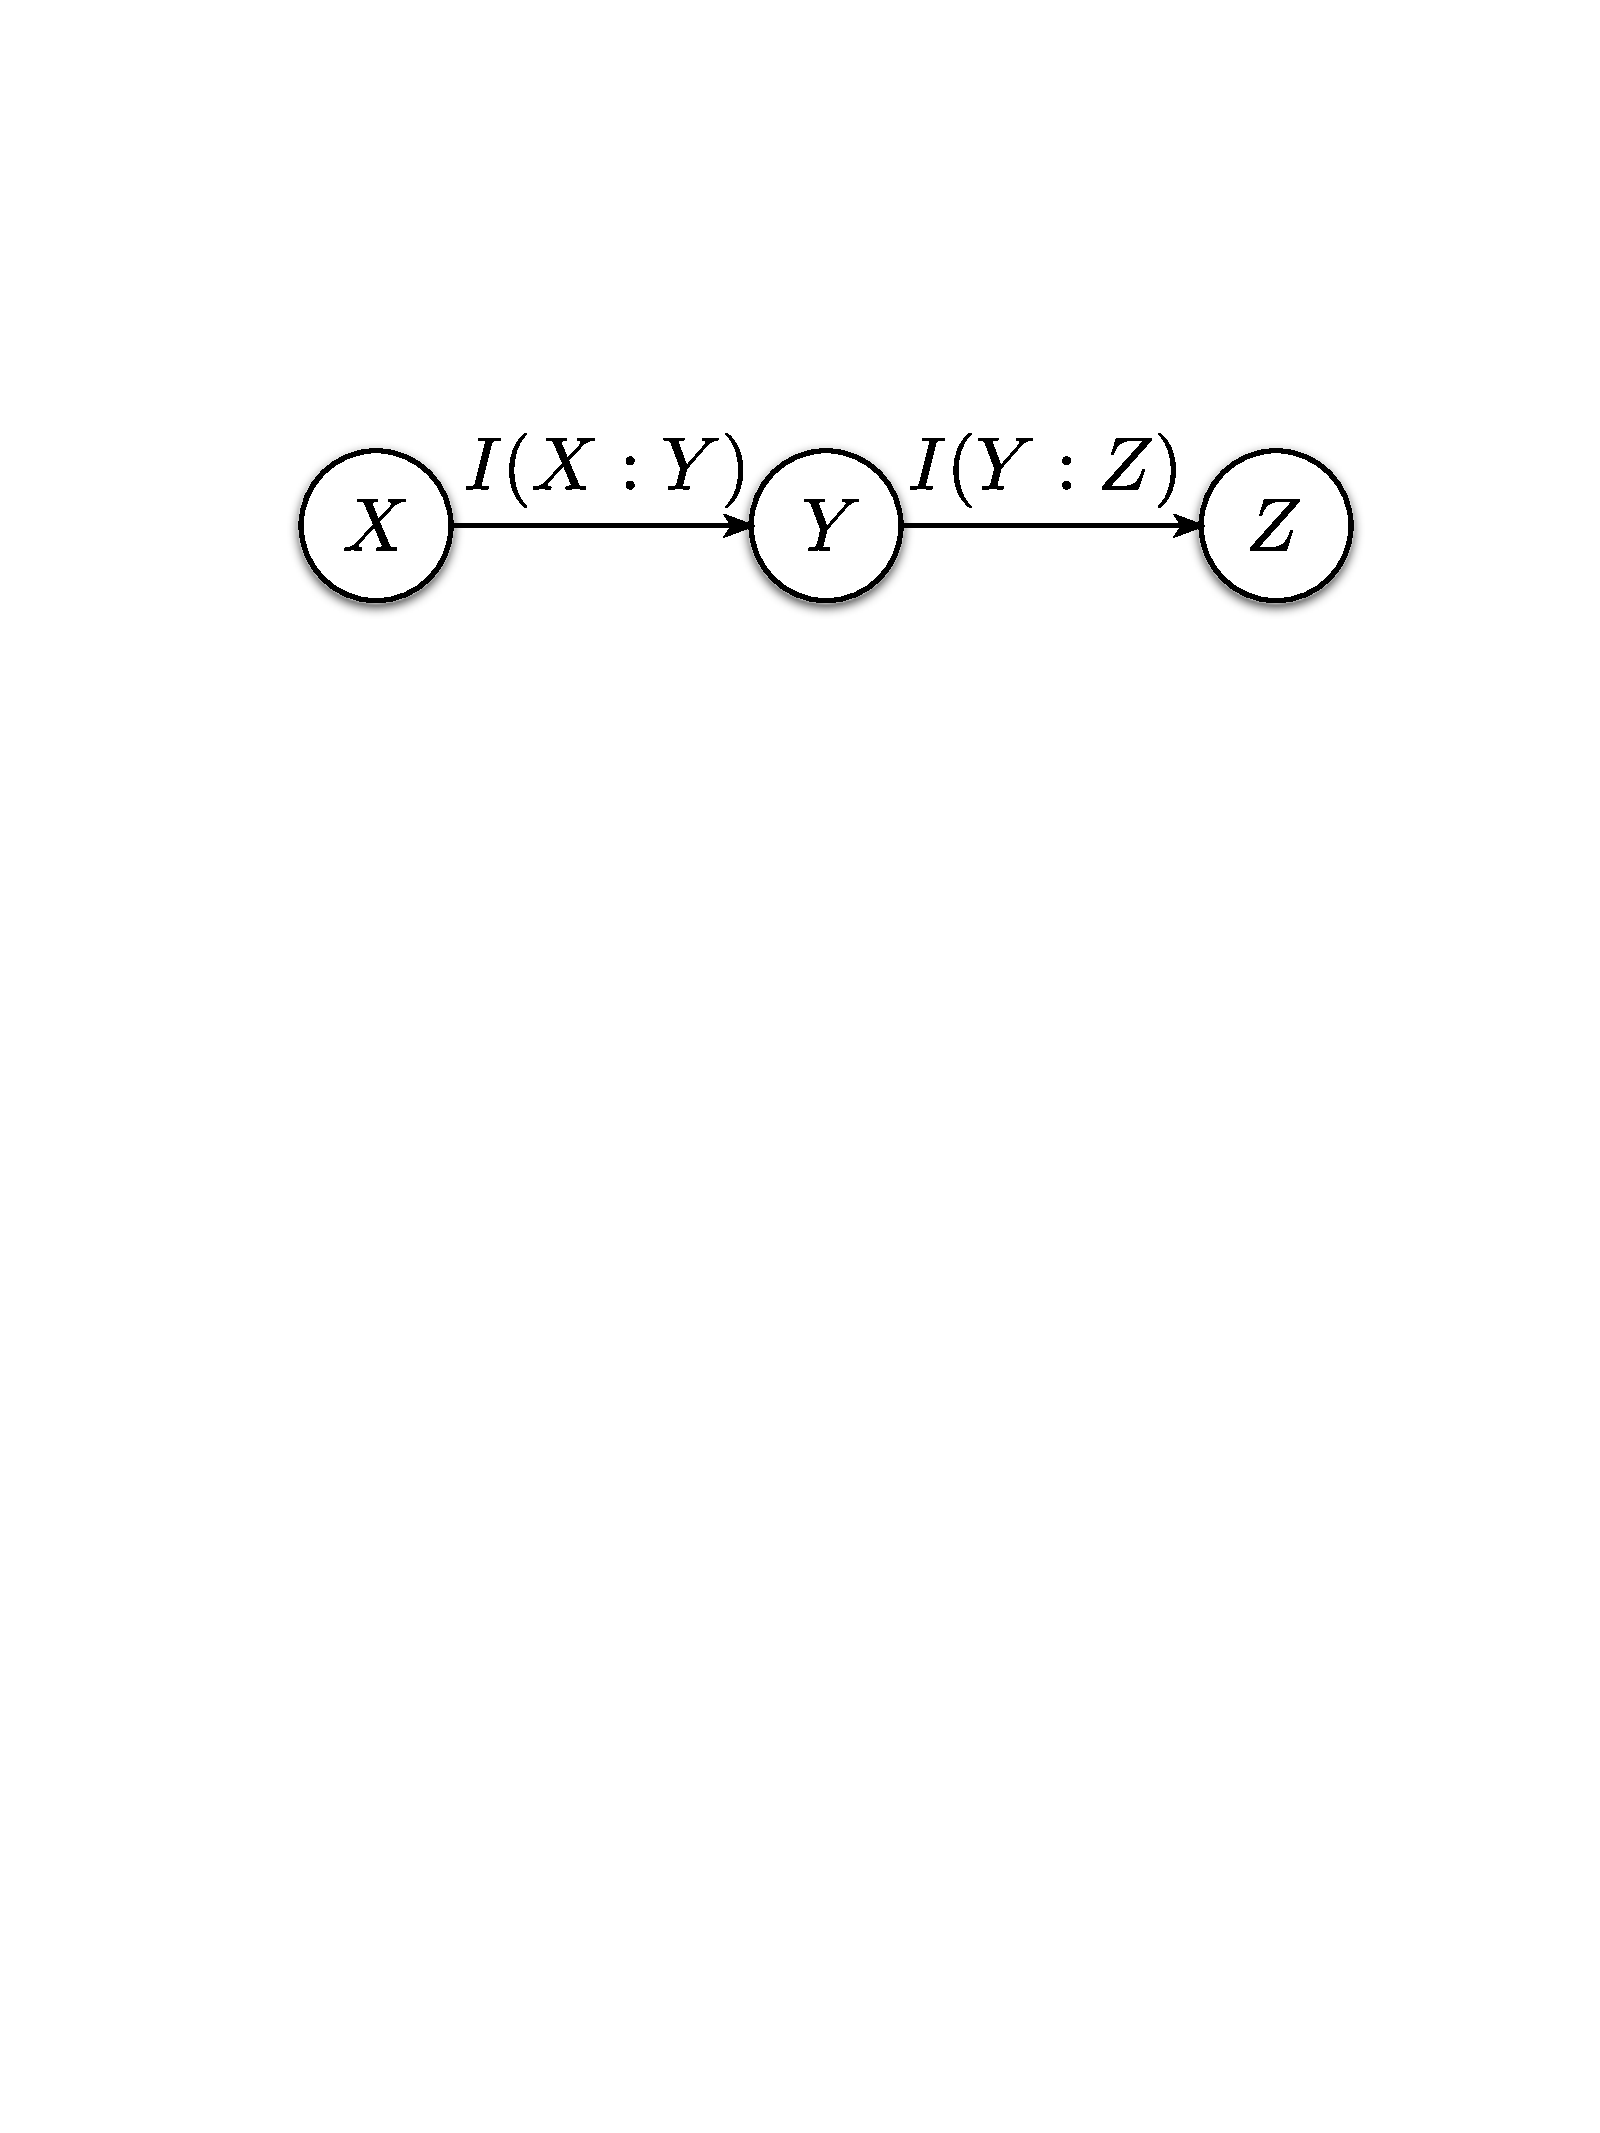
\includegraphics[clip=true, width=0.3\textwidth]{data_proc_ineq}
\captionspacefig \caption{\label{fig:data_proc_ineq}A sequence of events \mbox{$X\to Y\to Z$}. The data processing inequality states that the mutual information from beginning to end is upper-bounded by the mutual information between neighbouring stages, as per Eq.~(\ref{eq:data_proc_ineq}).}	
\end{figure}

The mutual information is defined as being between a particular known pair of states. Of course, in a quantum channel we have the flexibility to manipulate the input state and the measurement at the output. From this, we can then define the \textit{classical information of the channel}\index{Classical information of the channel}, $I_c(\hat\rho_{A,B})$ -- the maximum of the mutual information, optimised over \textit{all} possible measurement settings. Suppose $\hat\rho_{A,B}$ is shared between Alice and Bob, from which they would like to extract maximal correlations (i.e joint information). They measure using local measurement bases $\{\Lambda_A^x\}$ and $\{\Lambda_B^x\}$, yielding random variables $A$ and $B$. Their quantum mutual information of the channel is defined as,
\begin{align}
I_c(\hat\rho_{A,B}) = \max_{\rho,\{\Lambda_A^x\},\{\Lambda_B^x\}} I(A;B). 
\label{eq:quant_mut}
\end{align}

Eq.~\eqref{eq:quant_mut} quantifies the maximum amount of correlation that can be established between input and output states that can be achieved across the channel. This dictates the physical upper bound on the achievable bitrate (classical communication) or bandwidth of the channel.



% \paragraph{Quantum correlation measures}

We now move on to discuss quantum correlations. Whilst classical correlation measures have a clear operational meaning, quantum channel capacities are less so -- these quantities can be interpreted as how well the channel preserves the quantum state.

Analogous to the mutual information for classical systems is the \textit{coherent information} for quantum systems \cite{bib:PhysRevA.54.2629}, defined as,
\begin{align}\index{Coherent information}
I_\text{coh}(\hat\rho,\mathcal{E}) = S(\mathcal{E}(\hat\rho)) - S_e(\hat\rho,\mathcal{E}).
\label{eq:mutual_info_classical_single}
\end{align}
Here $S_e$ is the \textit{exchange entropy}, a measure of how much information is exchanged between the state $\hat\rho$ and the environment under the action of the process. Specifically, it is given by the entropy of the environment subsystem in Eq.~(\ref{eq:proc_environment}), after application of the channel. This yields the intuitive interpretation that the coherent information is the information contained in the evolved state, discounted by the amount lost to the environment. It can be alternatively written as,
\begin{align}
I(A\rangle B) = H(B)_{\hat\rho} - H(A,B)_{\hat\rho},
\end{align}
which we recognise as the negative of the conditional quantum entropy in Eq~\eqref{cond_quant_ent}.

The fact that the information quantity $H(A|B)$ can be negative is a signature of the fundamental difference between the laws of classical and quantum information.

